\begin{figure*}[hb]
  \centering

  \includegraphics[width=0.7\textwidth]{communication.svg.pdf}
  \caption{\textbf{Timeline of Communication From Frameworks to Mesos to Nodes}
  Time flows top to bottom, that is, communication arrows closer to the top
  happen before communication arrows closer to the bottom. When a framework
  enters the Mesos cluster, it will send a resourceRequest message to Mesos.
  Mesos then determines if it needs to perform revocation. If it does, then
  it will send killTasks messages to the nodes. Once the nodes have killed
  the tasks, it will then send a taskKilled message to Mesos. Finally, a
  Mesos sends a killedTask message to the corresponding framework to
  inform it that its task was killed.}
  \label{fig:communication}
\end{figure*}
